\section{Preprocesado de datos}

\subsection{DeepLabCut}\label{sec:DeepLabCut}

% DeepCatLab output
\begin{figure}[H]
  \centering
  \begin{subfigure}{0.45\textwidth}
    \centering
    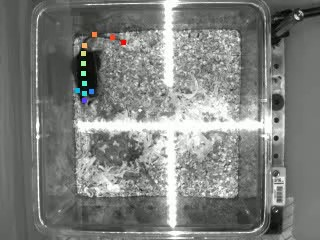
\includegraphics[width=\textwidth]{figures/deeplabcut-top-example-4128-2020-12-02-1-00-37.jpg}
    \caption{}
    \label{fig:deeplabcut-top-example}
  \end{subfigure}
  \begin{subfigure}{0.45\textwidth}
    \centering
    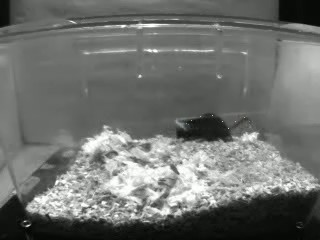
\includegraphics[width=\textwidth]{figures/deeplabcut-lateral-example-4128-2020-12-02-1-00-37.jpg}
    \caption{}
    \label{fig:deeplabcut-lateral-example}
  \end{subfigure}
  \caption[Salida de DeepLabCut.]
  {Salida de DeepLabCut del animal 4128 el 02-12-2020, 1:00:37. \ref{fig:deeplabcut-top-example} Video de la vista cenital de la caja. Los puntos sobre el animal son los dibujados por DeepCutLab para rastrear las partes del animal. \ref{fig:deeplabcut-lateral-example} Video de la vista lateral de la caja.}
  \label{fig:deeplabcut-outputexamples}
\end{figure}

\begin{table}[h]
  \centering
  \begin{tabular}{|c|c|c|c|c|c|c|}
  \hline
    & Nosex & Nosey & Noselikelihood & Headx & Heady & ... \\
  \hline
  0 & 136.165344 & 177.722496 & 0.000084 & 129.790253 & 174.772552 & ... \\
  1 & 162.032005 & 201.444756 & 0.942181 & 168.152061 & 202.420639 & ... \\
  2 & 156.297043 & 200.326378 & 0.000073 & 162.436028 & 203.156837 & ... \\
  3 & 155.370415 & 199.043297 & 0.000277 & 159.507599 & 200.199928 & ... \\
  4 & 149.272644 & 197.677170 & 0.000045 & 155.493912 & 198.814835 & ... \\
  ... & ... & ... & ... & ... & ... & ... \\
  \hline
  \end{tabular}
  \caption{Extracto del DataFrame de Pandas de los datos sin procesar de DeepLabCut.}
  \label{tab:df-example}
\end{table}

% Triangulations
\begin{figure}[H]
  \centering
  \begin{subfigure}{0.45\textwidth}
    \centering
    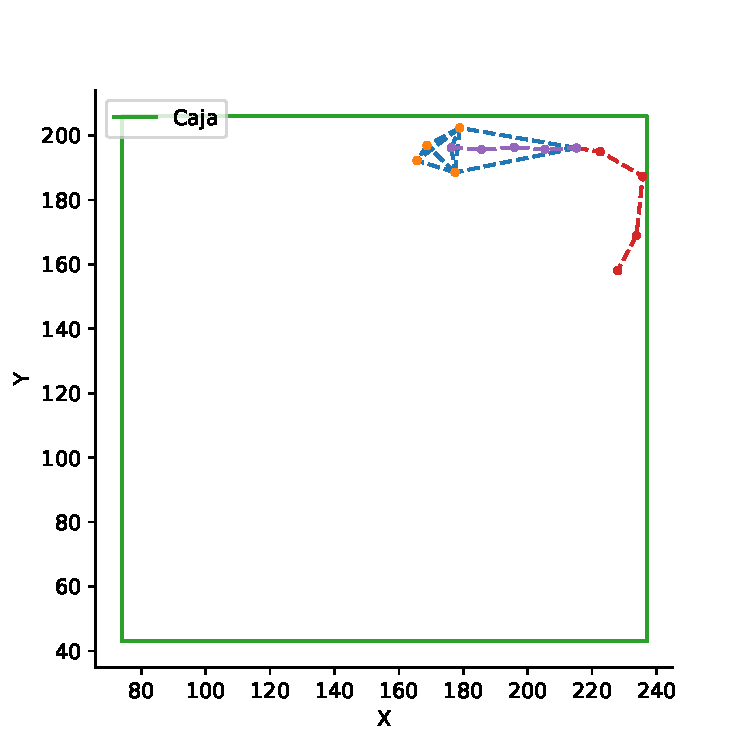
\includegraphics[width=\textwidth]{figures/triangulation-top-4128-2020-12-02.pdf}
    \caption{Vista cenital.}
  \end{subfigure}
  \begin{subfigure}{0.45\textwidth}
    \centering
    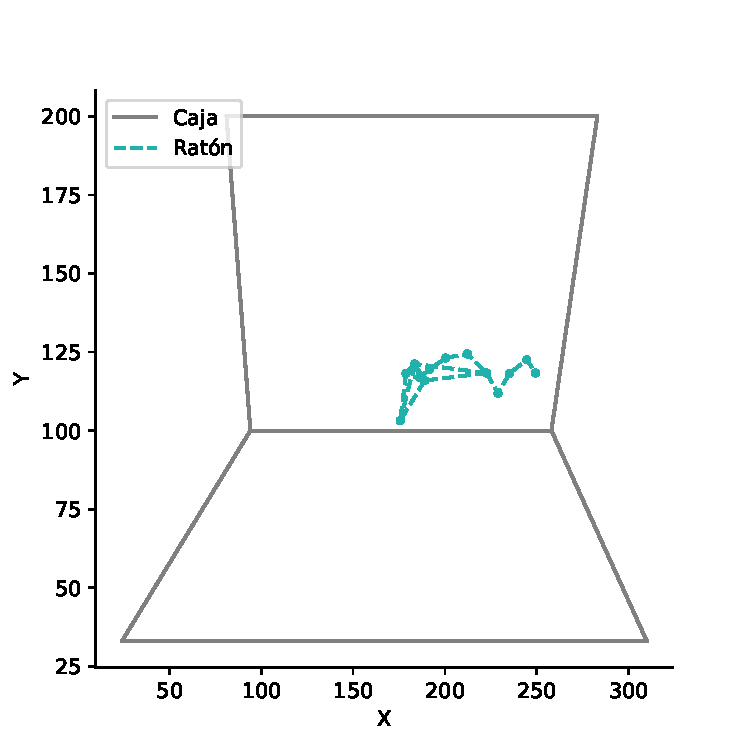
\includegraphics[width=\textwidth]{figures/triangulation-lateral-4128-2020-12-02.pdf}
    \caption{Vista lateral.}
  \end{subfigure}
  \caption{Triangulaciones de los puntos del animal 4128 el 02-12-2020, 1:00:37.}
  \label{fig:triangulations}
\end{figure}

\subsection{Filtrado e interpolación}

% Raw trayectory
\begin{figure}[H]
  \centering
  \begin{subfigure}{0.45\textwidth}
    \centering
    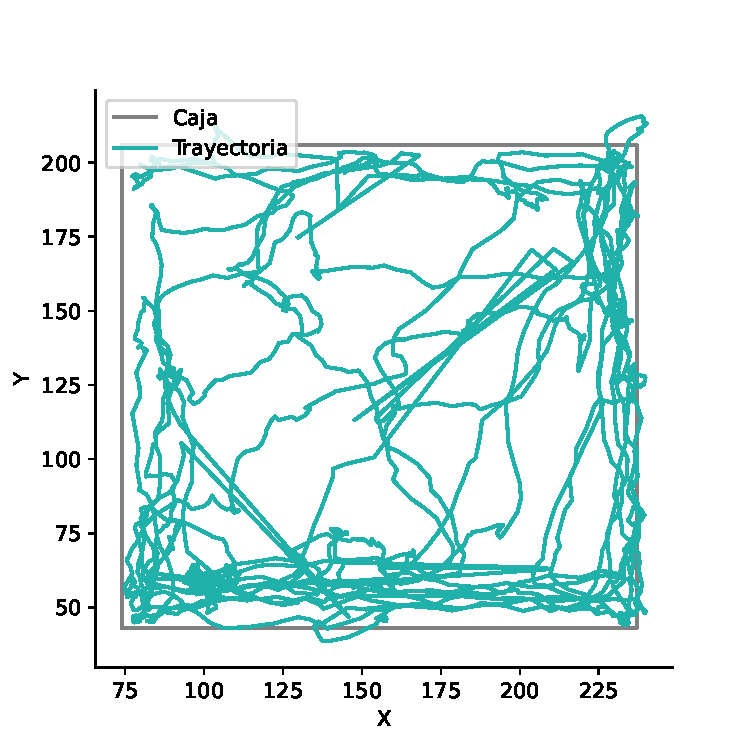
\includegraphics[width=\textwidth]{figures/raw-trayectory-top-4128-2020-12-02.pdf}
    \caption{Vista cenital.}
  \end{subfigure}
  \begin{subfigure}{0.45\textwidth}
    \centering
    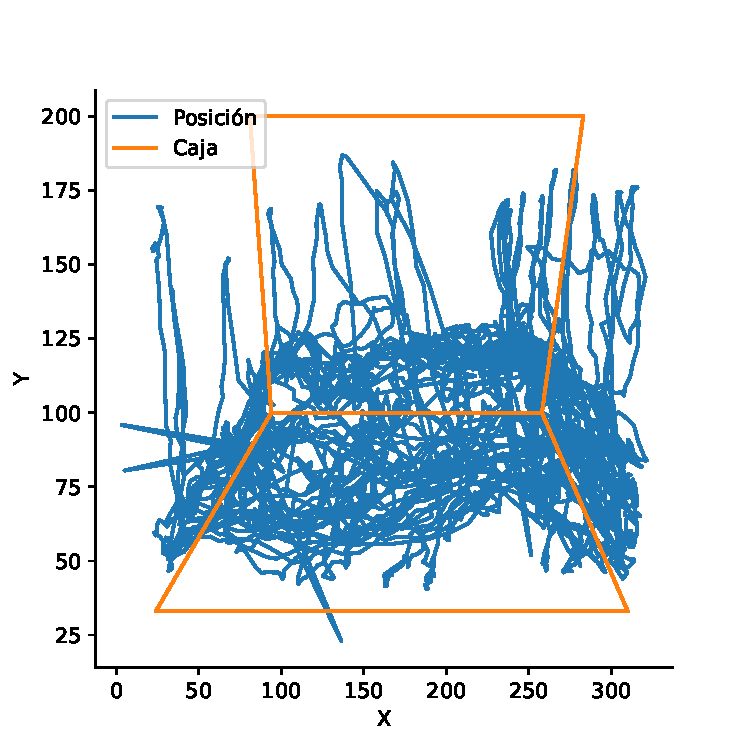
\includegraphics[width=\textwidth]{figures/raw-trayectory-lateral-4128-2020-12-02.pdf}
    \caption{Vista lateral.}
  \end{subfigure}
  \caption{Trayectoria de un punto de cabeza del animal 4128 el 02-12-2020.}
  \label{fig:raw-trayectories}
\end{figure}

% Filtered trayectory
\begin{figure}[H]
  \centering
  \begin{subfigure}{0.45\textwidth}
    \centering
    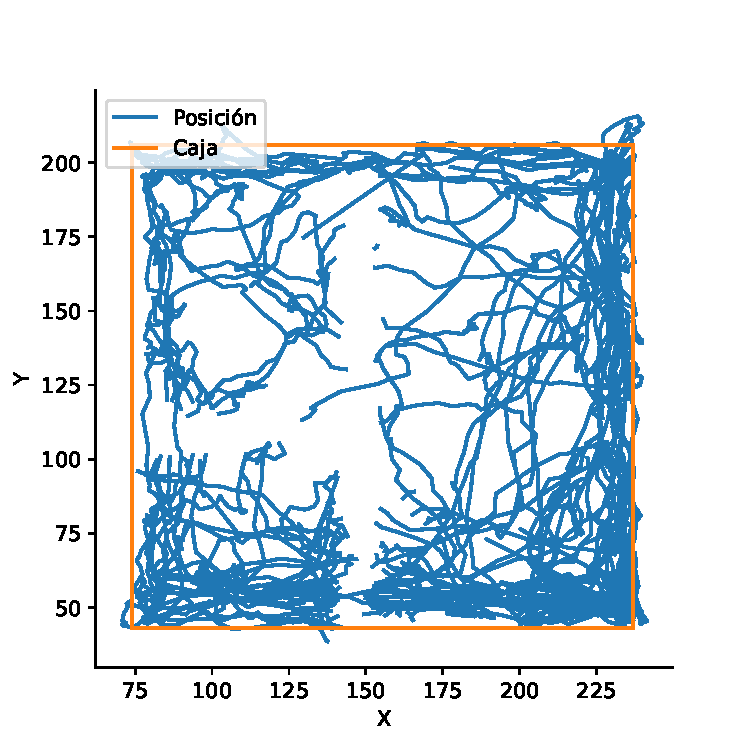
\includegraphics[width=\textwidth]{figures/filtered-trayectory-top-4128-2020-12-02.pdf}
    \caption{Vista cenital.}
  \end{subfigure}
  \begin{subfigure}{0.45\textwidth}
    \centering
    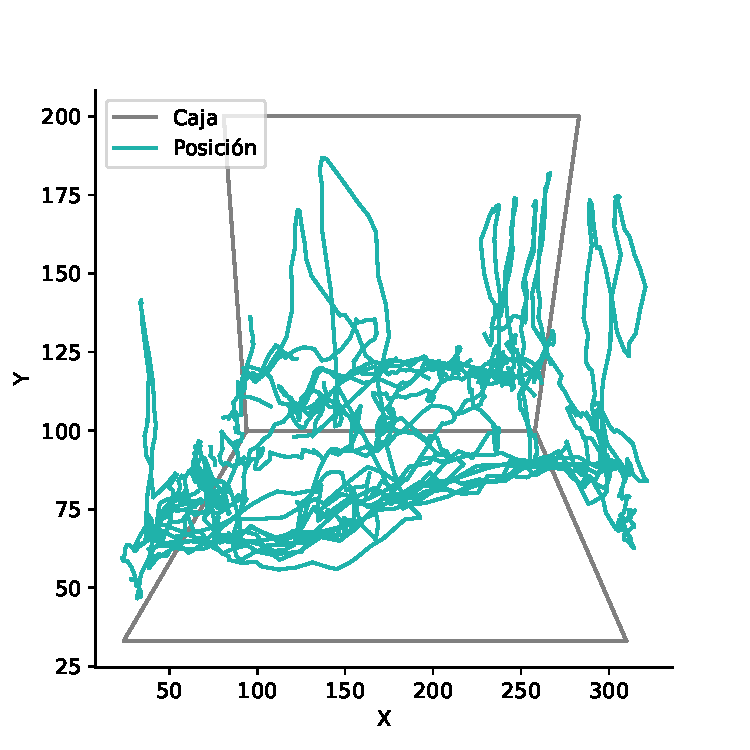
\includegraphics[width=\textwidth]{figures/filtered-trayectory-lateral-4128-2020-12-02.pdf}
    \caption{Vista lateral.}
  \end{subfigure}
  \caption{Trayectoria filtrada de un punto de la cabeza del animal.}
  \label{fig:filtered-trayectories}
\end{figure}

% Interpolated trayectory
\begin{figure}[H]
  \centering
  \begin{subfigure}{0.45\textwidth}
    \centering
    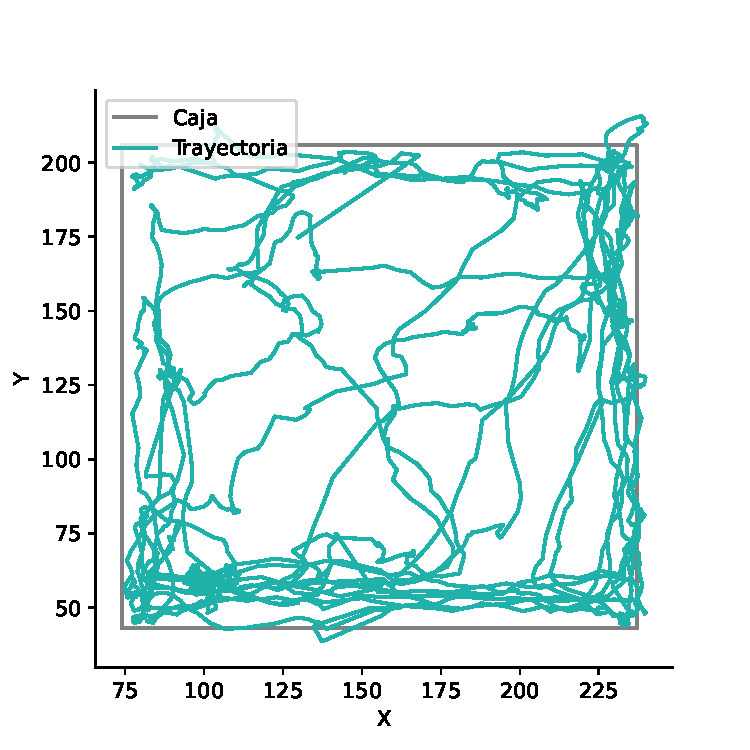
\includegraphics[width=\textwidth]{figures/interpolated-trayectory-top-4128-2020-12-02.pdf}
    \caption{Vista cenital.}
  \end{subfigure}
  \begin{subfigure}{0.45\textwidth}
    \centering
    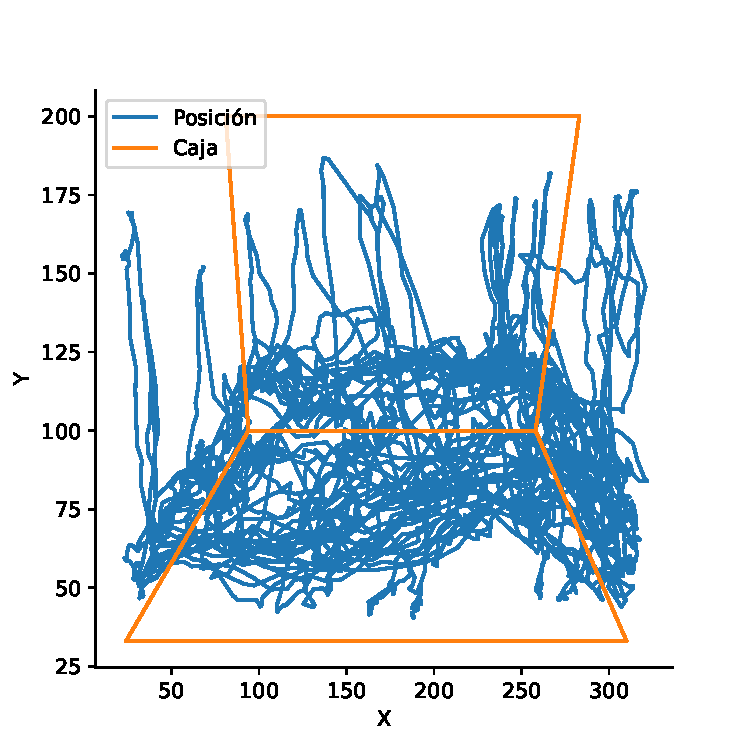
\includegraphics[width=\textwidth]{figures/interpolated-trayectory-lateral-4128-2020-12-02.pdf}
    \caption{Vista lateral.}
  \end{subfigure}
  \caption{Trayectoria interpolada de un punto de la cabeza del animal.}
  \label{fig:interpolated-trayectories}
\end{figure}


\subsection{Computo de variables a analizar}

\newpage
\section{Procesado de datos}

\subsection{Matriz de similitud}

\subsection{Agrupamiento por afinidad}

\subsection{Reducción de dimensionalidad para visualización}

\subsection{Entrenamiento de una red neuronal}


% \section{Pruebas \LaTeX}
% \subsection{Código}
% 
% \begin{mypython}[caption={Titulo del algoritmo/código.},label={alg:etiqueta}]
% def sum_list_limits_1(a, lower, upper):
%     if lower > upper:
%         return 0
%     else:
%         return a[upper] + sum_list_limits_1(a, lower, upper - 1)
% \end{mypython}
% 
% El código~\ref{alg:etiqueta} es un ejemplo en Python.
% 
% 
% 
% \begin{algorithm}[H]
% \begin{algorithmic}[1]
% \STATE $\forall i \in V$, \ let $i$ be an isolated community
% \STATE $o=permutation(V)$
% \FOR{$k \ \in \ o$}
% \STATE search in $A$ all the neighbours of $k$, $j$
% \STATE $\forall j$, calculate $\Delta Q_k(j)$ in matrix $\mathcal{M}$
% \STATE $j^*=\{ \ j \ | \ \Delta Q_k(j^*)=\max_j\{Q_k(j)\} \ \}$
% \IF{$\Delta Q_k(j^*)>0$}
% \STATE{Move node $k$ to $j^*$ 's community}
% \ELSE
% \STATE{$k$ remains in its community}
% \ENDIF
% \ENDFOR
% \end{algorithmic}\caption{\textit{Additional Louvain} \textbf{input}=$\left(A, \ \mathcal{M}\right)$ \textbf{output}=$P$}
% \label{alg:AdditionalLouvain}
% \end{algorithm}
% 
% En el algoritmo~\ref{alg:AdditionalLouvain} aparece un ejemplo en pseudocódigo.